\documentclass{article}
\usepackage{graphicx} % Required for inserting images
\usepackage{amsmath}

\usepackage[inkscapelatex=false,svgpath=./svg-inkscape/]{svg}




\title{Ponderful predictive models of nutrients report 
}
\author{Jing}
\date{September 2024}

\begin{document}

\maketitle

\section{Introduction}

Ponds play a vital role in local ecosystems, and understanding nutrient levels is critical for maintaining water quality and biodiversity. Predicting nutrient concentrations using environmental and biological factors is a complex task, given the heterogeneous nature of the data involved.

The present research outlines a comprehensive approach to model and predict total nitrogen (TN) and total phosphorous (TP) nutrient levels in ponds using various independent variables such as ponds’ physical characteristics including temperature, area, depth, animal intensity, hydro period length, utility land use variables. We developed predictive models that robustly estimates nutrient levels in ponds using a combination of environmental and biological predictors. These models account for the diverse distributions of the independent variables and optimize for predictive accuracy and interpret ability.

\section{Methods}

\subsection{Preprocessing and response variables selection}

We excluded upper outliers of TN (TN > 10 mg/L). Multicollinearity was assessed using the Variance Inflation Factor (VIF). Variables with VIF values less than 5 were retained, indicating low multicollinearity.


\subsection{Predictors normalization}

Prediction variables were normalized using \textit{bestNormalize}. As for heavily skewed land use variables (land use 5 meters and 500 meters), we applied a customized version of quantile normalization. The custom method deviates from the traditional quantile normalization technique[] by excluding zero values from the normalization process. We started by excluding zero values to avoid skewing the results. For the non-zero values in each column, ranks are computed. This involves assigning ranks to each value, where the smallest value gets the lowest rank and so on. The ranks then are transformed into quantiles using the inverse of the cumulative distribution function (CDF) of the normal distribution. This step standardizes the ranks to follow a normal distribution. The normalized values are then placed back into their original positions in the dataset, preserving the zeros and ensuring that the original structure of the data is maintained.

\subsection{Model Fitting}

We comprehensively examined the performance of fitting our dataset using Generalized Linear Model (GLM), Generalized Additive Model (GAM).

GLM \cite{mccullagh2019generalized} provides a flexible approach to modeling by allowing the response variable to follow different distributions from the exponential family and linking it to the explanatory variables via a linear predictor. The general form of a GLM is given by:
\[
g(\mu) = \beta_0 + \beta_1 x_1 + \beta_2 x_2 + \cdots + \beta_k x_k 
\]

where $g(\mu)$ is the link function, $\beta_0$ is the intercept, and $\beta_i$ are the coefficients for the explanatory variables $x_i$.

In a GAM\cite{guisan2002generalized}, the relationship between the response variable  $Y  $ and the explanatory factors is expressed as:
\[
g(\mu) = \beta_0 + f_1(x_1) + f_2(x_2) + \cdots + f_k(x_k)
\]

where:

-  $g(\mu)  $ is the link function that connects the expected value  $\mu  $ of the response variable  $Y  $ to the linear predictor.
-  $\beta_0  $ is a constant term (intercept).
-  $f_i(x_i)  $ represents a smoothing function that describes the relationship between  $g(\mu)  $ and the  $i  $-th explanatory factor  $x_i  $.
-  $k  $ is the number of explanatory factors included in the model.

GAMM further extends GAMs by incorporating random effects to account for variability due to hierarchical or clustered data structures. The GAMM formula includes both fixed effects and random effects:

\[
g(\mu) = \beta_0 + f_1(x_1) + f_2(x_2) + \cdots + f_k(x_k) + 1 \text{random effect}) 
\]

where $g(\mu)$ is the link function, $\beta_0$ is the constant term, $f_i(x_i )$ are smooth functions, and ($1|random effect$) represents the random effects component.


To determine the most appropriate model, we utilized adjusted R-squared, generalized cross-validation (GCV),  AIC (Akaike information criterion) and deviance explained as criteria. Within each model, the significance of each factor was evaluated using F-statistics and p-values

GLMM Mariginal and 

\section{Results}


\subsection{European-Mediterranean region}


\begin{figure}[h]
    \centering
    \includesvg[width=0.75\columnwidth]{temp_euromedi/ponderful_OUTPUT_rmd_publicationtp_euromedi_glm_predictors.svg}
    \caption{Your Caption}
    \label{fig:your-label}
\end{figure}




\end{document}
width=1\linewidthtemp_euromedi/tn_ctn_gam_diagnostics.png

\subsection{3.1 Preditive models of TP}

\subsubsection{3.1.1 GAM model}

Do we have area again but not country as random effect? Could we have the plots for forest and depth? I still think 9 predictors is too much. Model interpretation is complicated and I'm afraid of overfitting. Is there a way to get simpler models? I've been reading here you can also use AIC, BIC or other methods to compare models to be sure adding more predictors improves the model. Did you use that with GAM as well? GAM yields the \textbf{final} best TP model as follows with adjusted R-square of 0.318, deviance explained 52\%, GCV of 0.83:



\begin{eqnarray}
\text{TP} &\sim & \, s(\text{Aquatic\_500, k=2}) + s(\text{Cropland\_500}) + \text{Forest\_500} \\\nonumber
&&+ s(\text{Pastures\_and\_open\_nature\_500,k=4}) \\
&&+ s(\text{Animals\_cont}, k = 7) + s(\text{Area}) + \text{Depth} \\
&&+ s(\text{bio1, k=9}) + s(\text{bio4, k=3}) + s(\text{bio12, k=4}) + s(\text{bio12})
\end{eqnarray}

The intercept term is estimated as -1.54 ($p < 2e-16$), along with two predictors (\texttt{Forest\_500} and \texttt{Depth}) that contribute linearly to TP. All predictors with statistically significant smooth terms ($p$-value $< 0.05$) include \texttt{Aquatic\_500}, 
\texttt{Pastures.and.open.nature\_500}, \texttt{Animals\_cont}, \texttt{Area.t}, \texttt{bio1.t}, \texttt{bio4.t}, and \texttt{bio12.t}. These variables exhibit non-linear effects on the response variable, indicating their important role in the model.

\begin{figure}
 \centering
 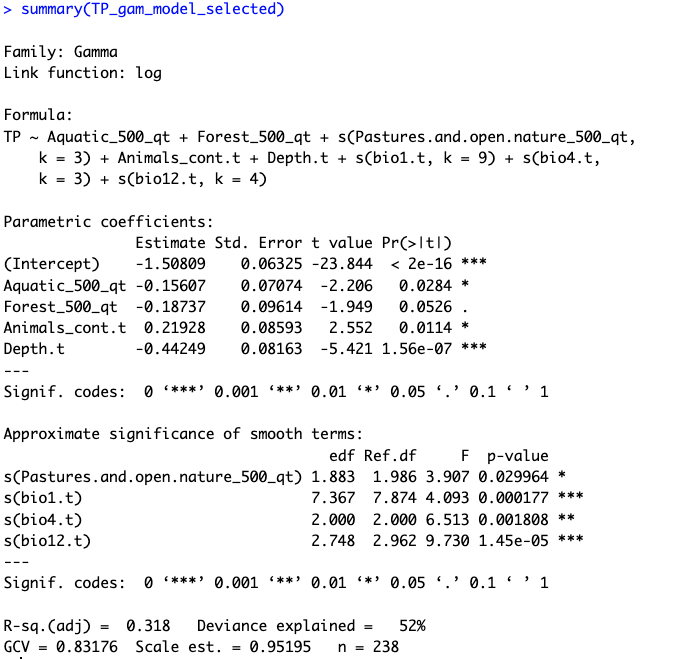
\includegraphics[width=1\linewidth]{tp_gam_sum.png}
 \caption{Enter Caption}
 
\end{figure}
\begin{figure}
 \centering
 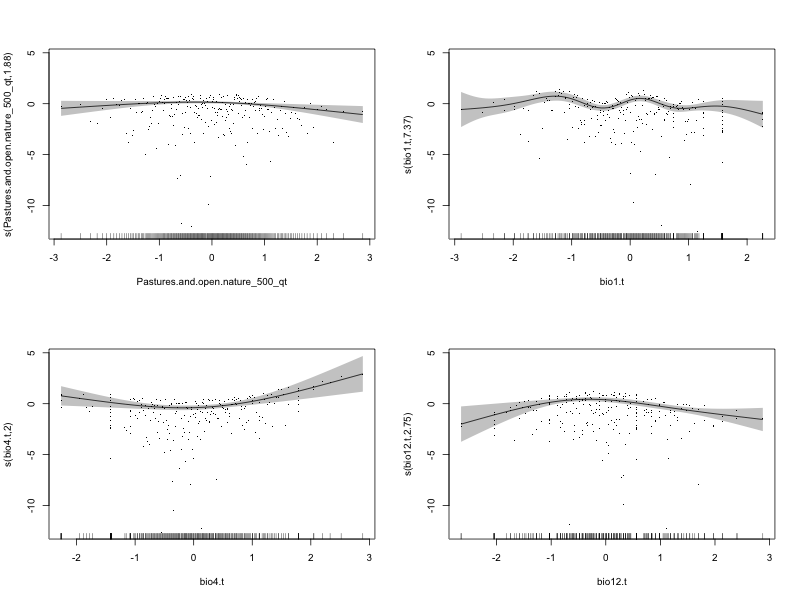
\includegraphics[width=1\linewidth]{tp_gam_predictors.png}
 \caption{Enter Caption}
 
\end{figure}
\begin{figure}
 \centering
 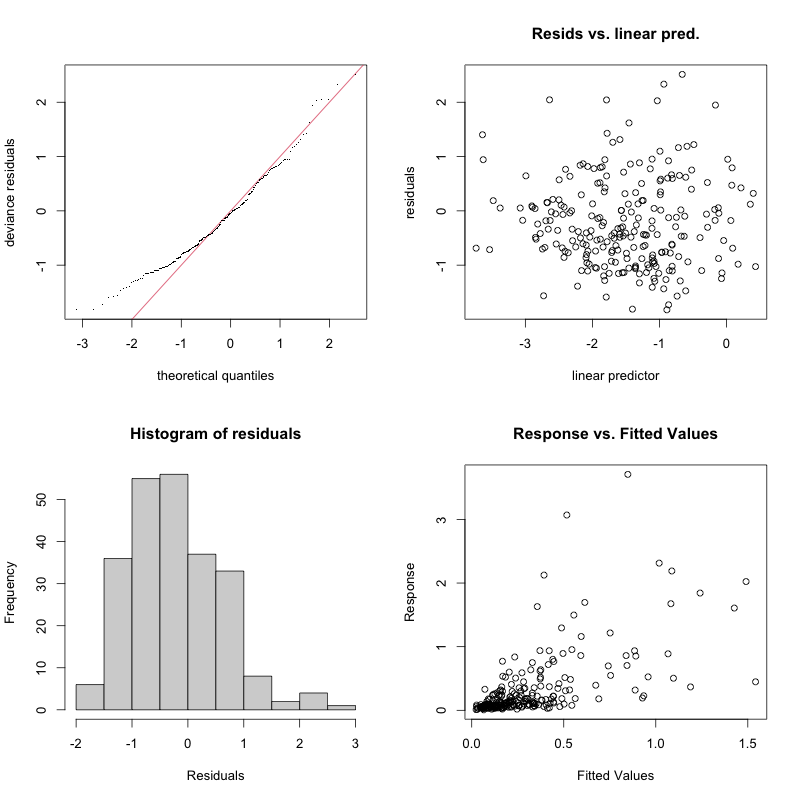
\includegraphics[width=1\linewidth]{tp_gam_diagnostics.png}
 \caption{Enter Caption}
 
\end{figure}

Updates Sep 17th by adding select =TRUE to gam, variables can be penalized to zero this way we can reduce amounts of predictors in the model efficiently 





\subsubsection{3.1.2 GLM model}

Fitting GLM results in a selection of seven variables explaining (deviance of 23.7\%). Adjusted R-squared: 0.2139 

\begin{eqnarray}
\text{E(TP)} =0.32 \, \text{-0.06 Natural\_5} \text{-0.90 Forest\_500} & 
 \text{-0.08 Pastures\_and\_open\_nature\_500,} \\
& \text{+0.11 Animals\_cont} \text{-0.15 Depth} \\
&- \text{0.08 bio5} \text{-0.12 bio12}
\end{eqnarray}

\begin{figure}
 \centering
 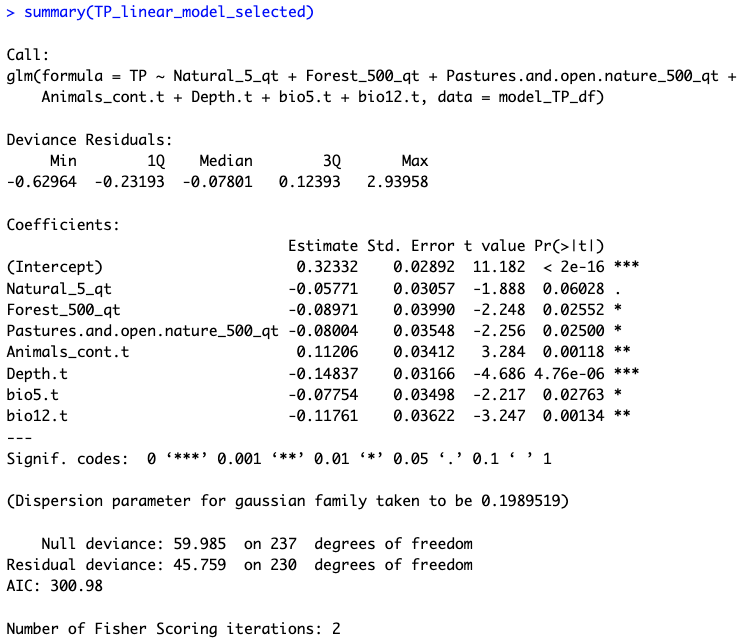
\includegraphics[width=\linewidth]{./tp_glm_sum.png}
 \caption{Enter Caption}
 
\end{figure}

\begin{figure}
 \centering
 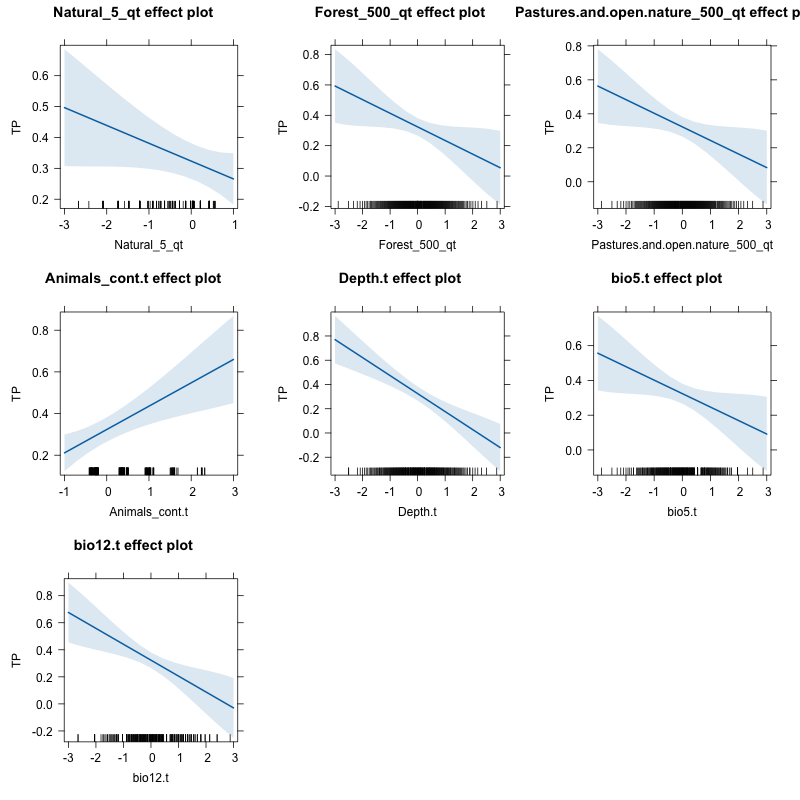
\includegraphics[width=1\linewidth]{tp_glm_predictors.png}
 \caption{Enter Caption}
 
\end{figure}
\begin{figure}
 \centering
 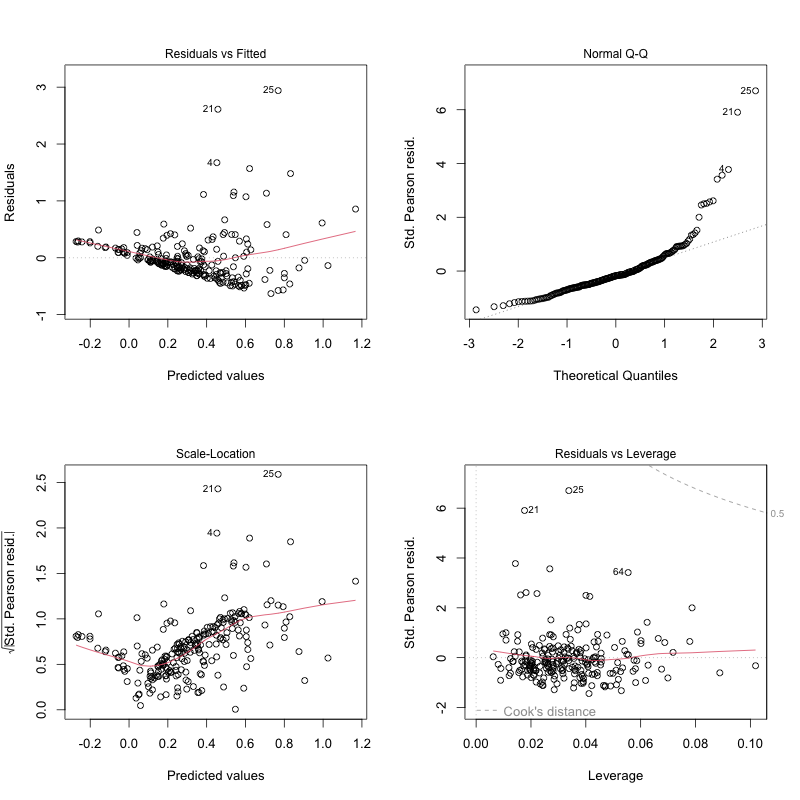
\includegraphics[width=1\linewidth]{tp_glm_diagnostics.png}
 \caption{Enter Caption}
 
\end{figure}

\subsubsection{3.1.3 TP model per bio climatic region}

\textbf{Mediterranean} GAM

\begin{figure}
 \centering
 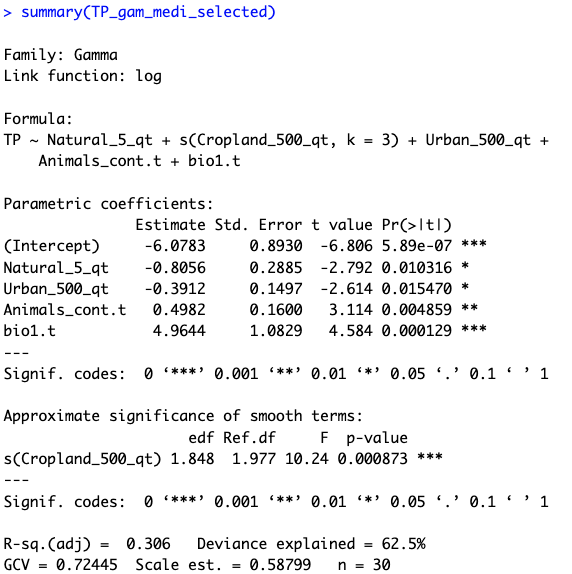
\includegraphics[width=0.75\linewidth]{tp_medi_gam_sum.png}
 \caption{Enter Caption}
 
\end{figure}
\begin{figure}
 \centering
 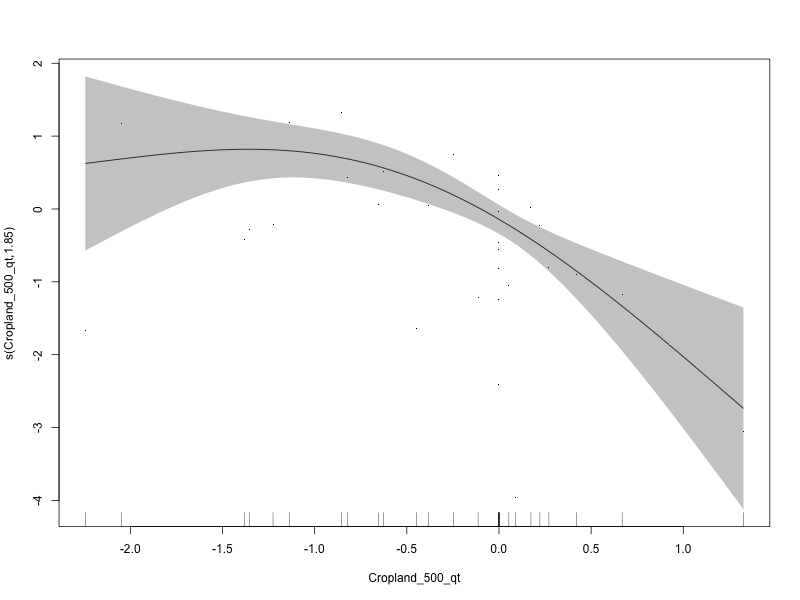
\includegraphics[width=1\linewidth]{tp_medi_gam_predictors.png}
 \caption{Enter Caption}
 
\end{figure}
\begin{figure}
 \centering
 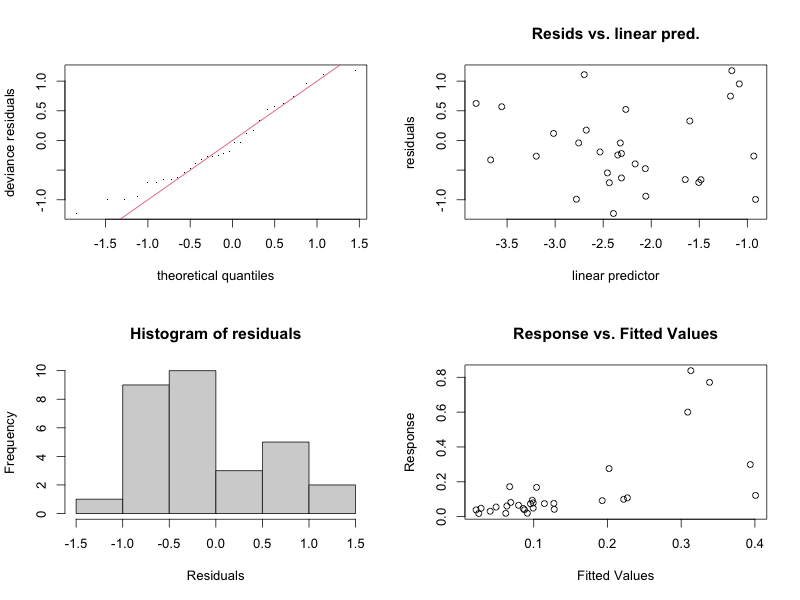
\includegraphics[width=1\linewidth]{tp_medi_gam_diagnostics.png}
 \caption{Enter Caption}
 
\end{figure}
Medi GLM deviance 0.2647506 Adjusted R-squared: 0.1471 

\begin{figure}
 \centering
 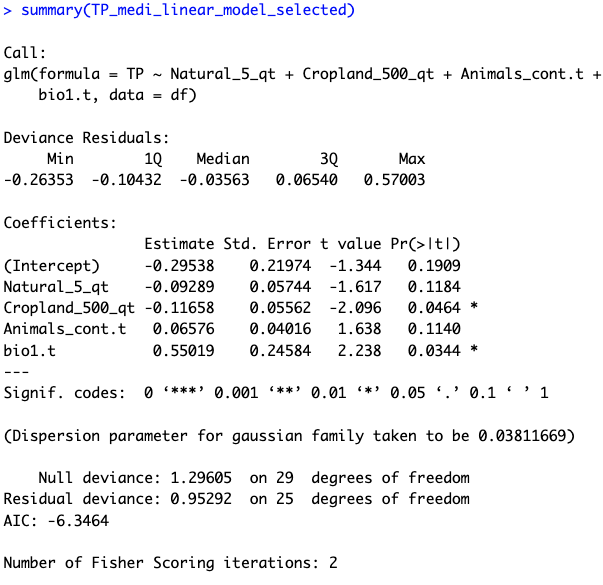
\includegraphics[width=0.75\linewidth]{tp_medi_glm_sum.png}
 \caption{Enter Caption}
 
\end{figure}
\begin{figure}
 \centering
 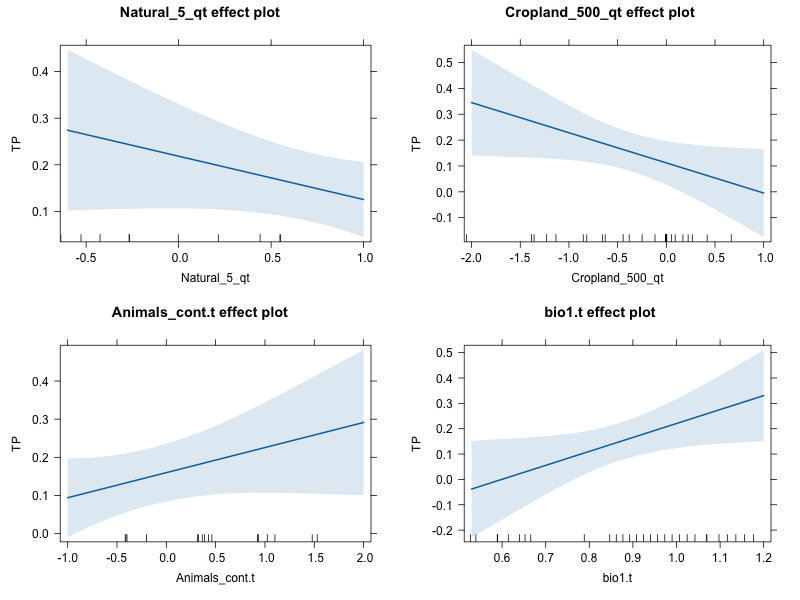
\includegraphics[width=1\linewidth]{tp_medi_glm_predictors.png}
 \caption{Enter Caption}
 
\end{figure}
\begin{figure}
 \centering
 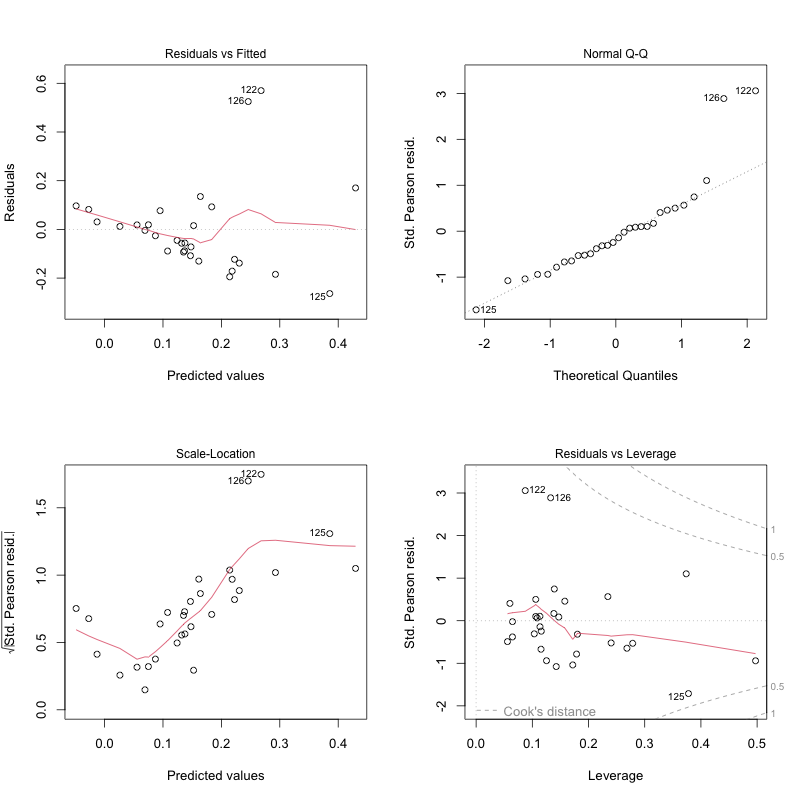
\includegraphics[width=1\linewidth]{tp_medi_glm_diagnostics.png}
 \caption{Enter Caption}
 
\end{figure}


\textbf{Continental} GAM (to improve)

\begin{figure}
 \centering
 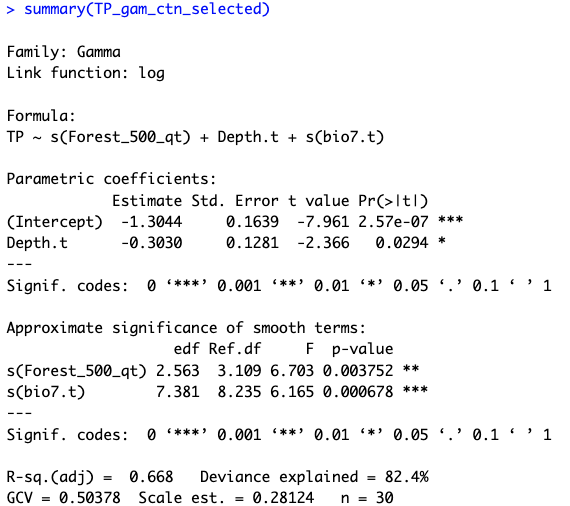
\includegraphics[width=0.75\linewidth]{tp_ctn_gam_sum.png}
 \caption{Enter Caption}
 
\end{figure}

\begin{figure}
 \centering
 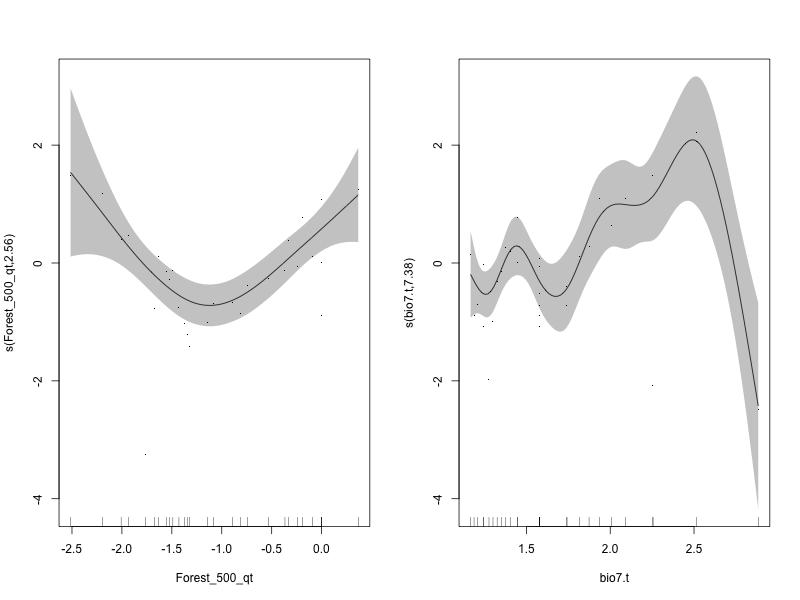
\includegraphics[width=1\linewidth]{tp_ctn_gam_predictors.png}
 \caption{Enter Caption}
 
\end{figure}
\begin{figure}
 \centering
 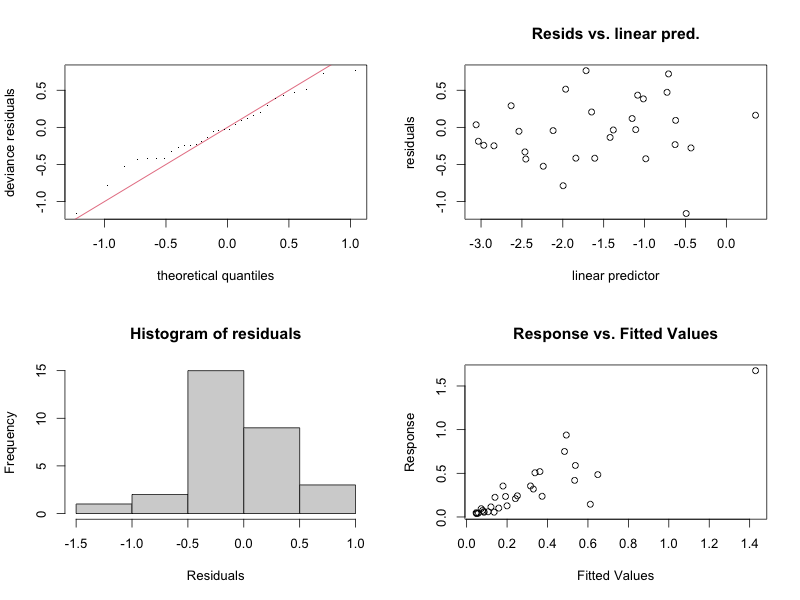
\includegraphics[width=1\linewidth]{tp_ctn_gam_diagnostics.png}
 \caption{Enter Caption}
 
\end{figure}

CTN GLM Adjusted R-squared: 0.2616 DEV 0.3379564
\begin{figure}
 \centering
 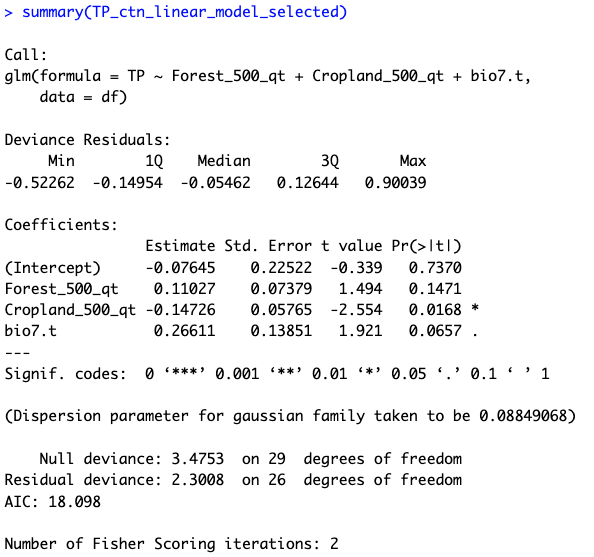
\includegraphics[width=1\linewidth]{tp_ctn_glm_sum.png}
 \caption{Enter Caption}
 
\end{figure}
\begin{figure}
 \centering
 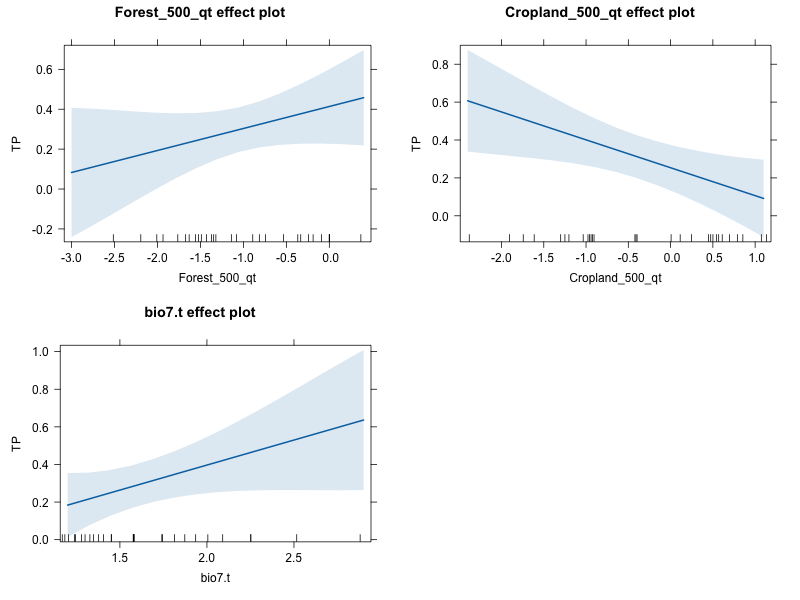
\includegraphics[width=1\linewidth]{tp_ctn_glm_predictors.png}
 \caption{Enter Caption}
 
\end{figure}
\begin{figure}
 \centering
 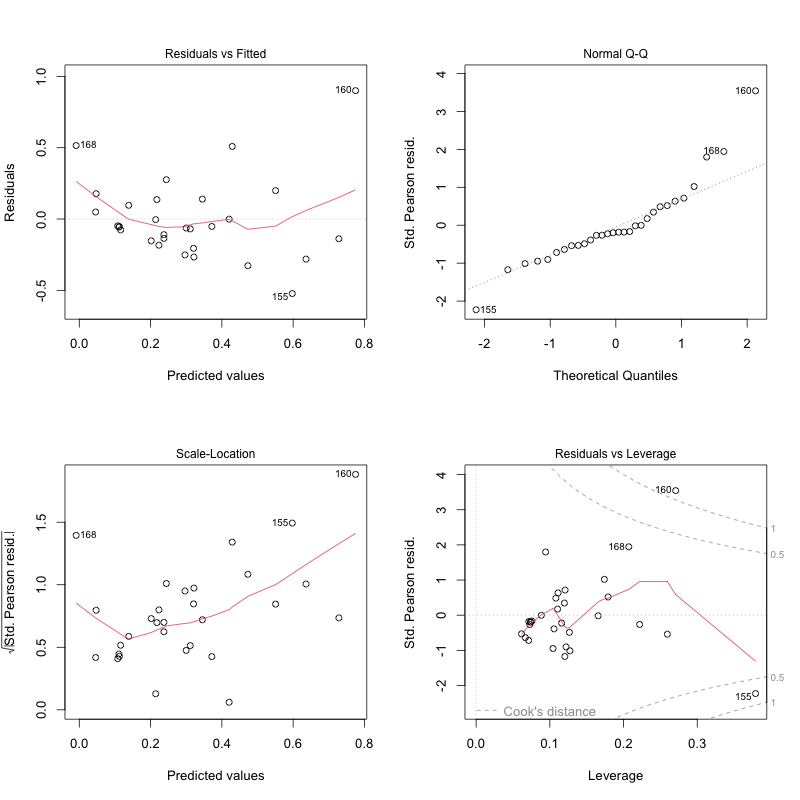
\includegraphics[width=1\linewidth]{tp_ctn_glm_diagnostics.png}
 \caption{Enter Caption}
 
\end{figure}

\textbf{Temperate} GAM 
\begin{figure}
 \centering
 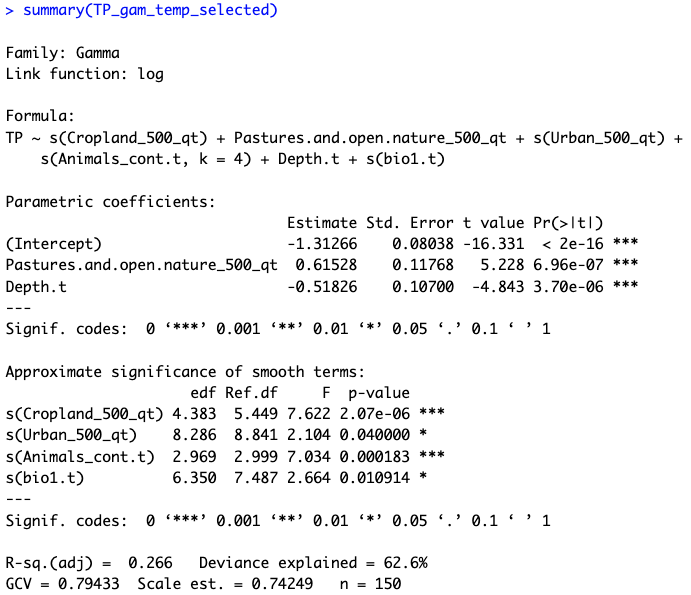
\includegraphics[width=0.75\linewidth]{tp_temp_gam_sum.png}
 \caption{Enter Caption}
 
\end{figure}
\begin{figure}
 \centering
 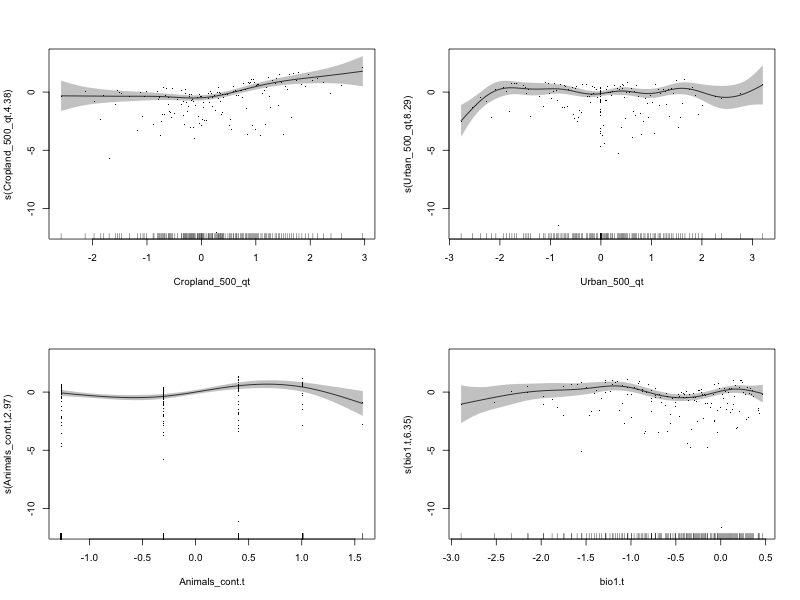
\includegraphics[width=1\linewidth]{tp_temp_gam_predictors.png}
 \caption{Enter Caption}
 
\end{figure}
\begin{figure}
 \centering
 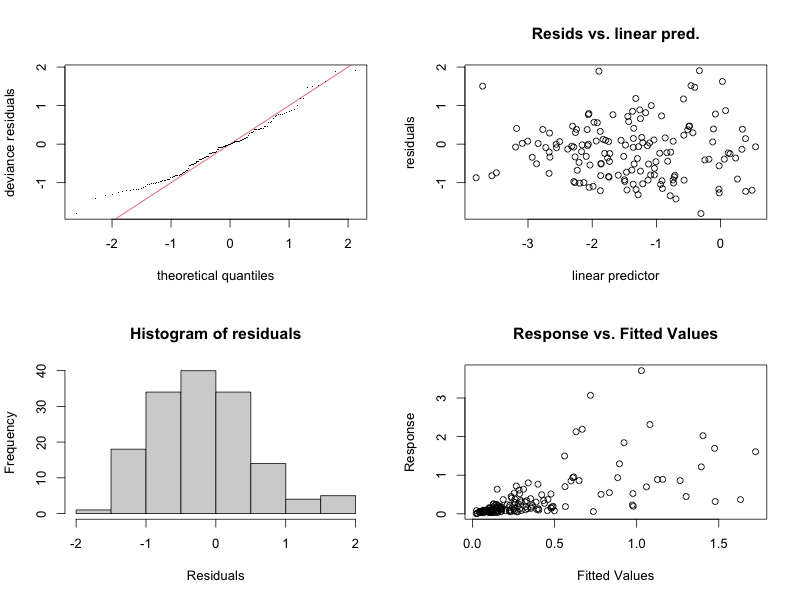
\includegraphics[width=1\linewidth]{tp_temp_gam_diagnostics.png}
 \caption{Enter Caption}
 
\end{figure}

temp GLM Adjusted R-squared: 0.2221 DEV 0.2429848
\begin{figure}
 \centering
 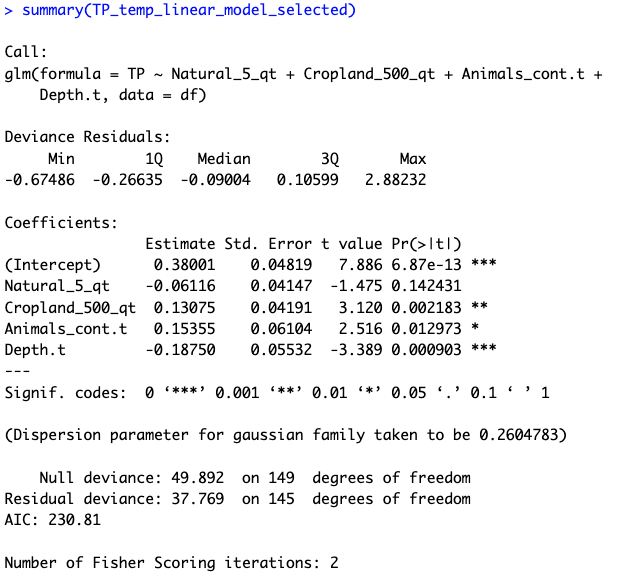
\includegraphics[width=0.75\linewidth]{tp_temp_glm_sum.png}
 \caption{Enter Caption}
 
\end{figure}
\begin{figure}
 \centering
 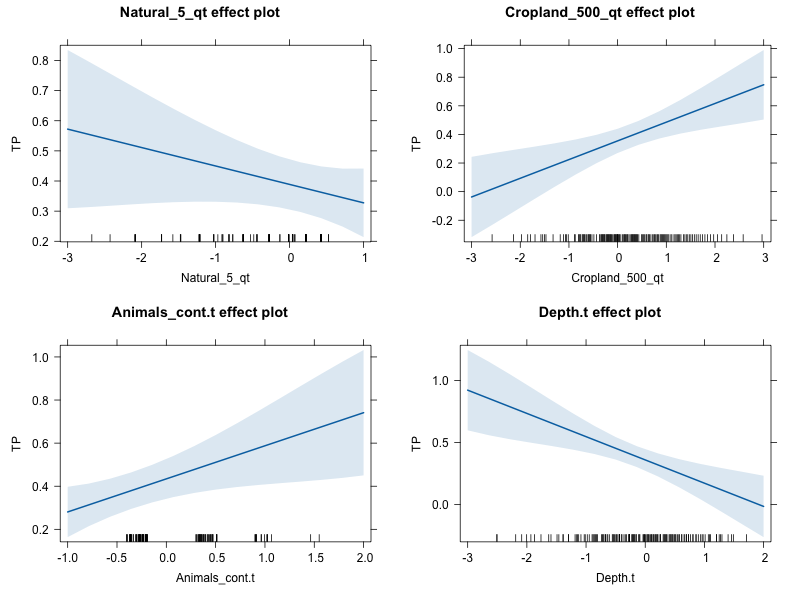
\includegraphics[width=1\linewidth]{tp_temp_glm_predictors.png}
 \caption{Enter Caption}
 
\end{figure}
\begin{figure}
 \centering
 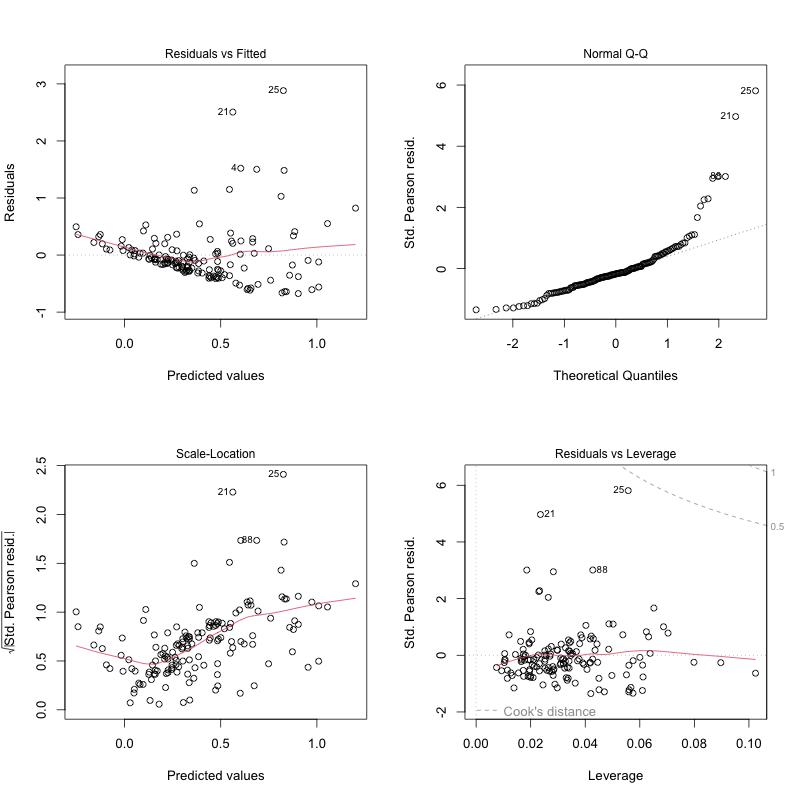
\includegraphics[width=1\linewidth]{tp_temp_glm_diagnostics.png}
 \caption{Enter Caption}
 
\end{figure}

\textbf{Subtropical GAM}
\begin{figure}
 \centering
 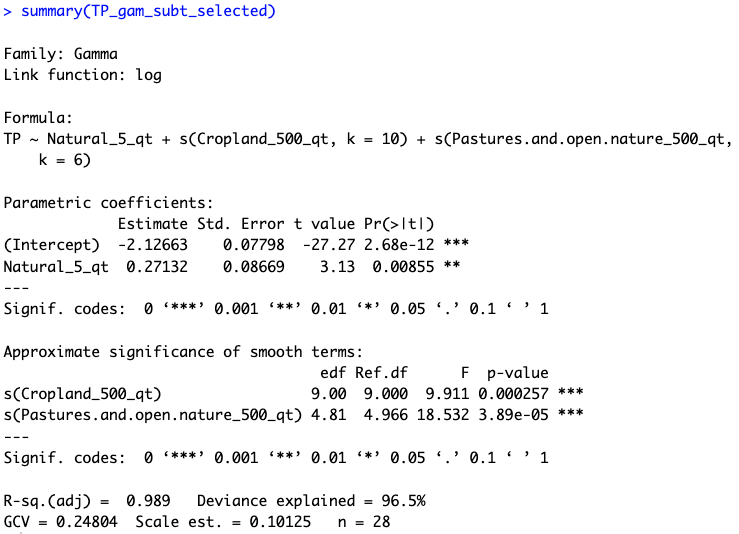
\includegraphics[width=0.75\linewidth]{tp_subt_gam_sum.png}
 \caption{Enter Caption}
 
\end{figure}

\begin{figure}
 \centering
 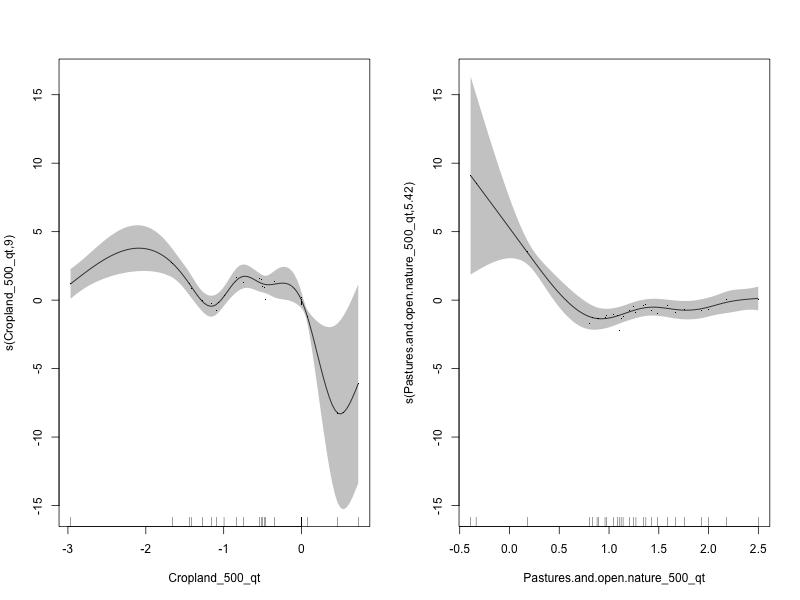
\includegraphics[width=1\linewidth]{tp_subt_predictors.png}
 \caption{Enter Caption}
 
\end{figure}

\begin{figure}
 \centering
 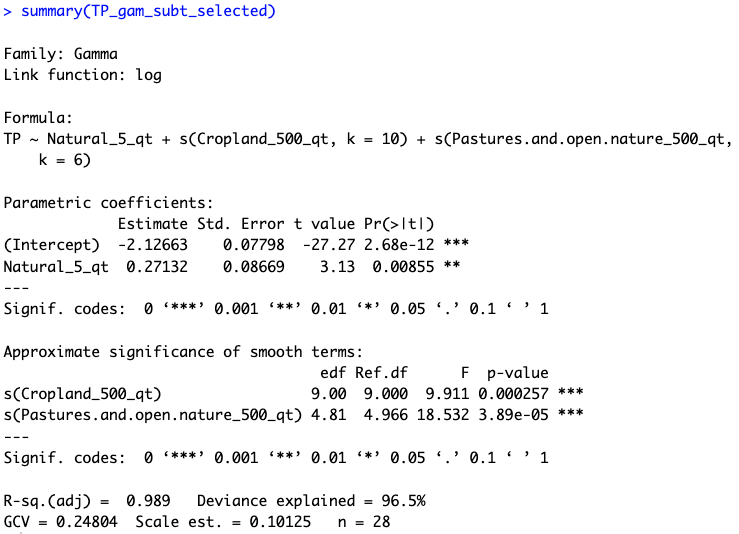
\includegraphics[width=1\linewidth]{tp_subt_gam_sum.png}
 \caption{Enter Caption}
 
\end{figure}

Subp GLM Adjusted R-squared: 0.487 DEV 0.5250319
\begin{figure}
 \centering
 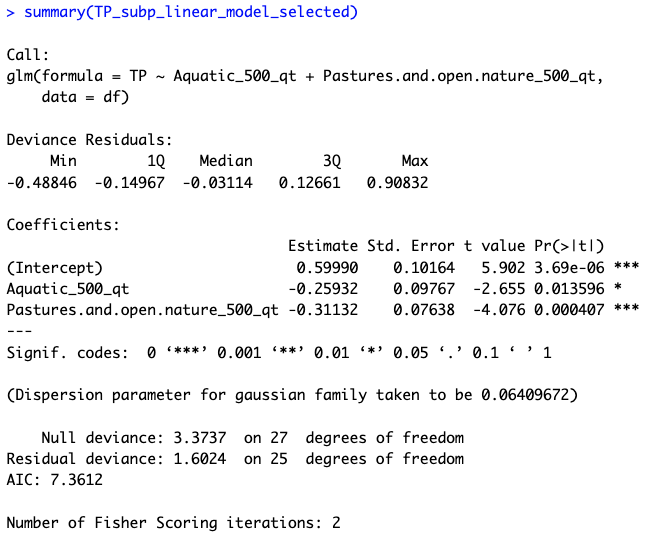
\includegraphics[width=0.75\linewidth]{tp_subp_glm_sum.png}
 \caption{Enter Caption}
 
\end{figure}

\begin{figure}
 \centering
 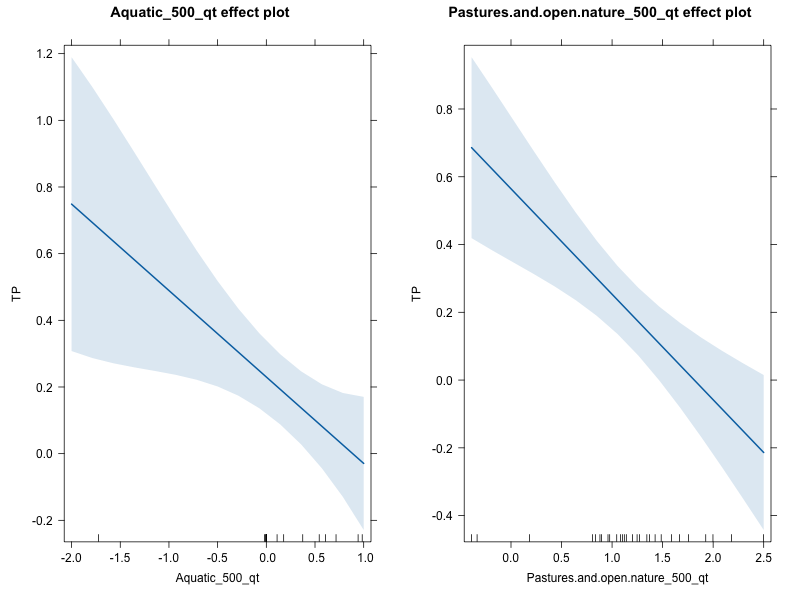
\includegraphics[width=1\linewidth]{tp_subp_glm_predictors.png}
 \caption{Enter Caption}
 
\end{figure}
\begin{figure}
 \centering
 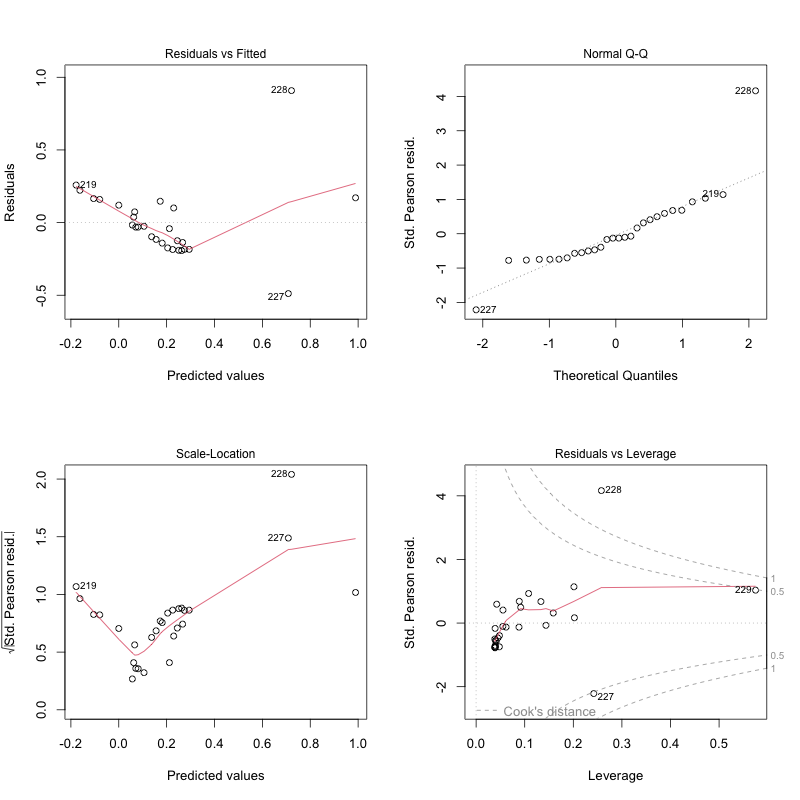
\includegraphics[width=1\linewidth]{tp_subp_glm_diagnostics.png}
 \caption{Enter Caption}
 
\end{figure}

GAMM yields the best TN model as follows with adjusted R-square of 0.37, deviance expalined 58\%, GCV of 0.31:
\begin{equation}
\begin{split}
\text{TN} \sim & \, + s(\text{Forest\_500}) \\
&+ s(\text{Pastures\_and\_open\_nature\_500}) \\
&+ s(\text{Depth}) \\
&+ s(\text{Country},'re')
\end{split}
\end{equation}

The intercept term is estimated as 0.46 ($p <0.001$). All predictors with statistically significant smooth terms ($p-\mathrm{value} < 0.05$) include \texttt{Forest\_500}, \texttt{Pastures.and.open.nature500}, \texttt{Area.t}, \texttt{Depth}, \texttt{Country}, \texttt{bio4.t}, and \texttt{bio12.t}. These variables exhibit non-linear effects on the response variable, indicating their important role in the model.

\subsection{3.2 Predictive models of TN}
GAM in Figure \ref{fig:tn_gam_sum}
\begin{figure}
 \centering
 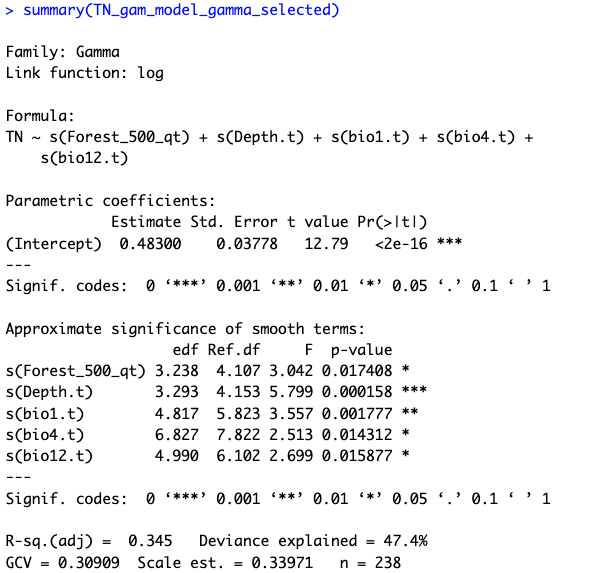
\includegraphics[width=0.75\linewidth]{tn_gam_sum.png}
 \caption{Enter Caption}
 \label{fig:tn_gam_sum}
\end{figure}
\begin{figure}
 \centering
 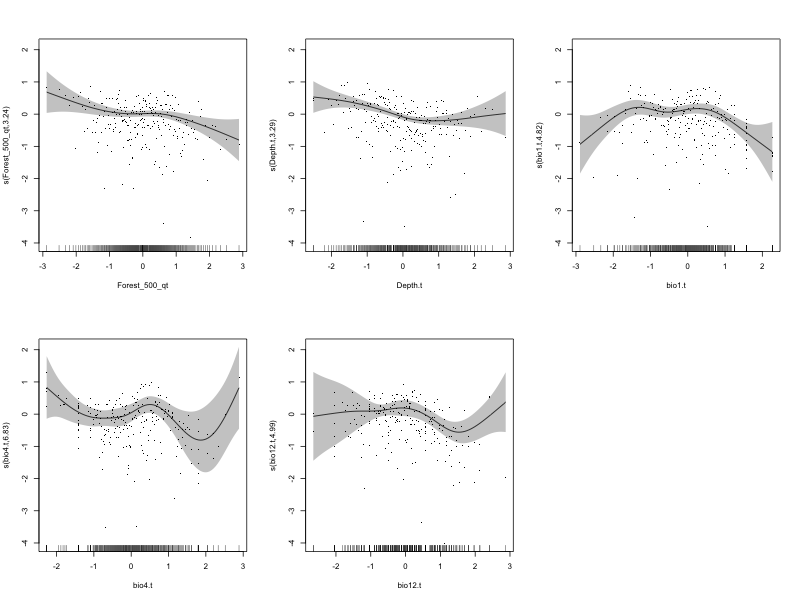
\includegraphics[width=1\linewidth]{tn_gam_predictors.png}
 \caption{Enter Caption}
 \label{fig:tn_gam_predictors}
\end{figure}
\begin{figure}
 \centering
 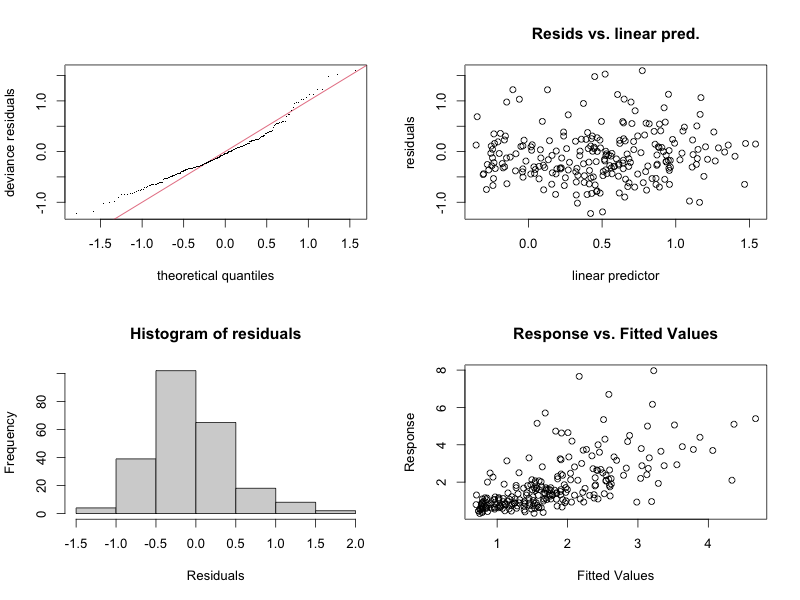
\includegraphics[width=1\linewidth]{tn_gam_diagnostics.png}
 \caption{Enter Caption}
 \label{fig:tn_gam_diagnostics}
\end{figure}

\subsubsection{3.2.2 GLM model}

GLM model selected using stepAIC reveals a linear relationship between TN and depth(p<0.001), bio4, area, forest\_500, bio5, (p<0.05) and pastures.and.open.nature\_500 with an intercept of 1.81 (p<2e-16). It explained 23.4\% of deviance and has an adjusted R-squared of 0.2137.

\begin{figure}
 \centering
 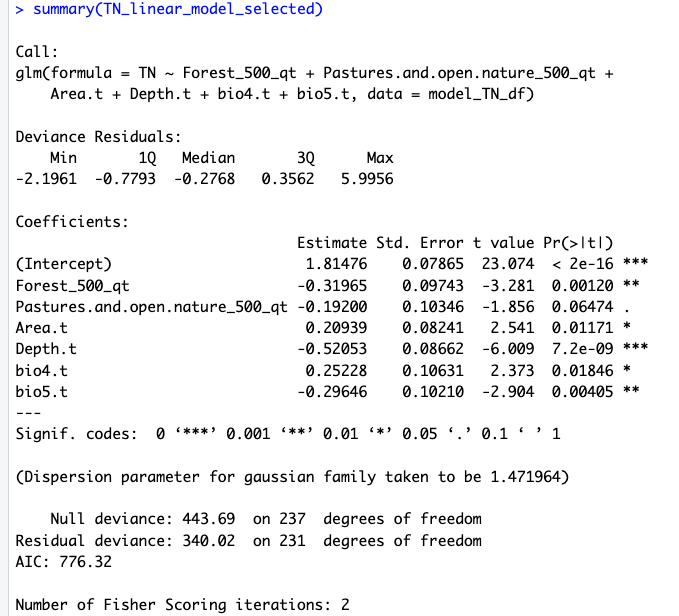
\includegraphics[width=1\linewidth]{tn_glm_step_sum.png}
 \caption{Enter Caption}
\end{figure}
\begin{figure}
 \centering
 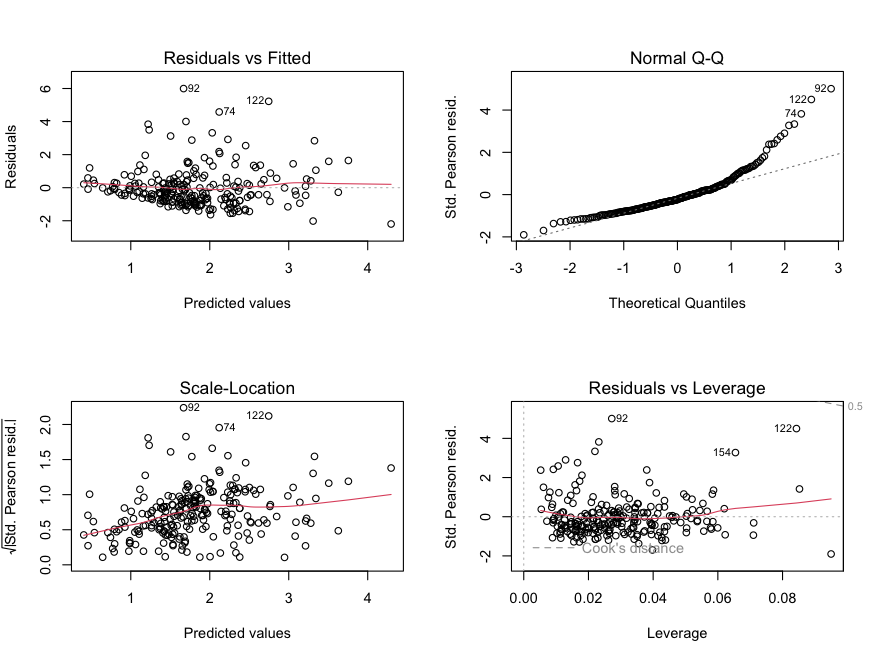
\includegraphics[width=1\linewidth]{tn_glm_step_diagnostics.png}
 \caption{Enter Caption}
 
\end{figure}
\begin{figure}
 \centering
 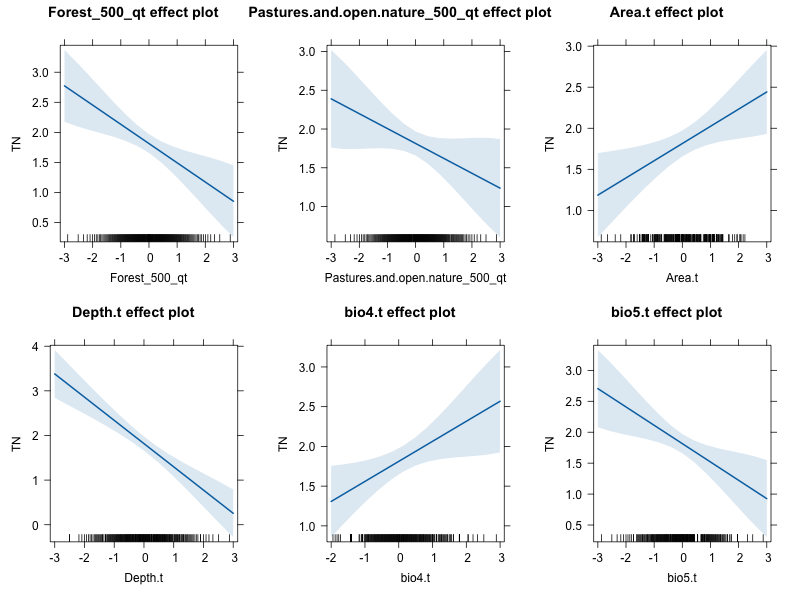
\includegraphics[width=1\linewidth]{tn_glm_step_predictors.png}
 \caption{Enter Caption}
\end{figure}
\subsubsection{3.2.1 Temperate regions}

GAM
\begin{figure}
 \centering
 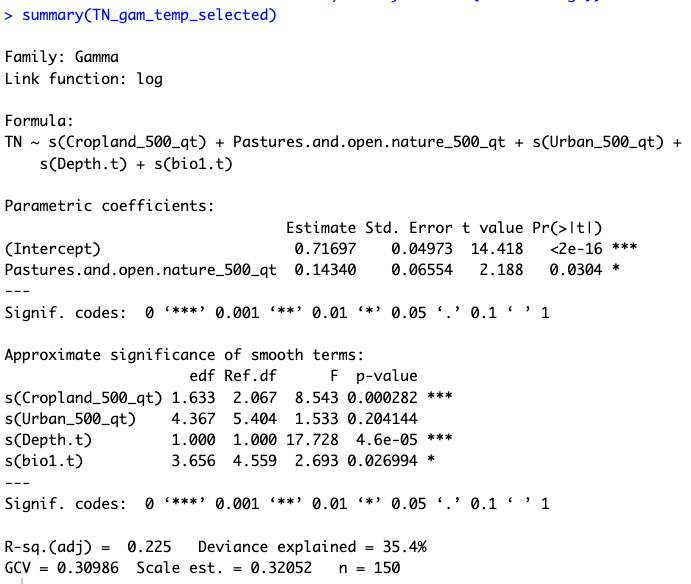
\includegraphics[width=0.75\linewidth]{tn_temp_gam_sum_noselected.png}
 \caption{Enter Caption}
 
\end{figure}
\begin{figure}
 \centering
 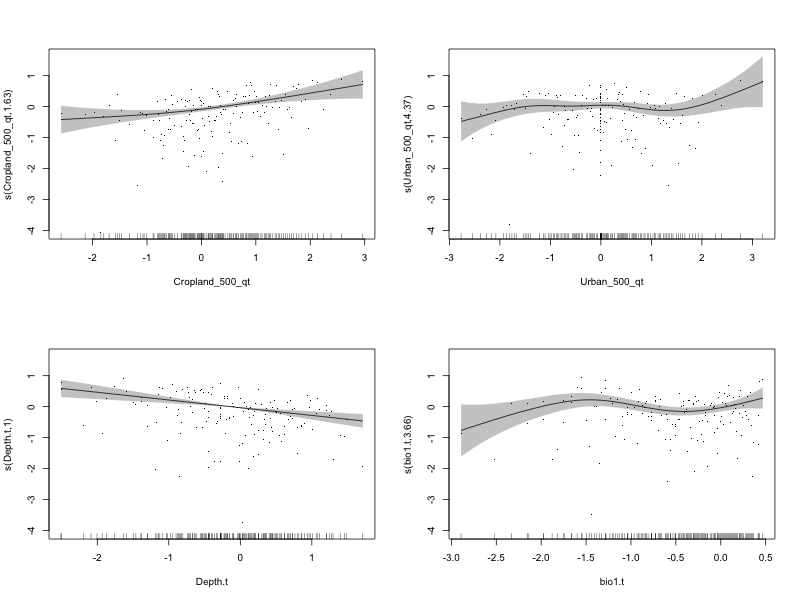
\includegraphics[width=1\linewidth]{tn_temp_gam_predictors.png}
 \caption{Enter Caption}
 
\end{figure}

\begin{figure}
 \centering
 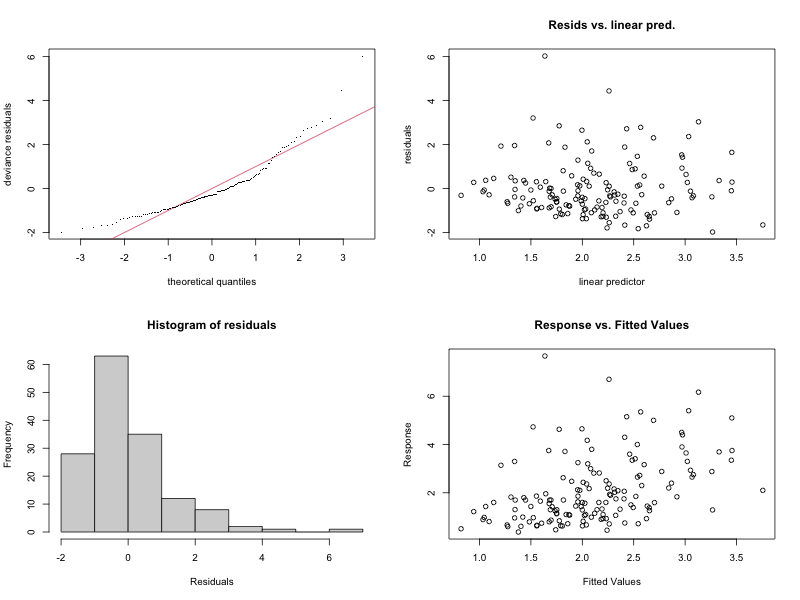
\includegraphics[width=1\linewidth]{tn_tempt_gam_diagnostics.png}
 \caption{Enter Caption}
 
\end{figure}

GLM Adjusted R-squared: 0.1649 DEV 0.1761583
\begin{figure}
 \centering
 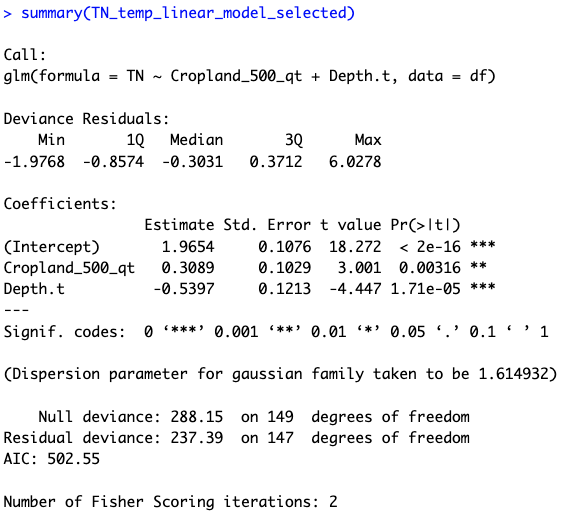
\includegraphics[width=0.75\linewidth]{tn_temp_glm_sum.png}
 \caption{Enter Caption}
 
\end{figure}
\begin{figure}
 \centering
 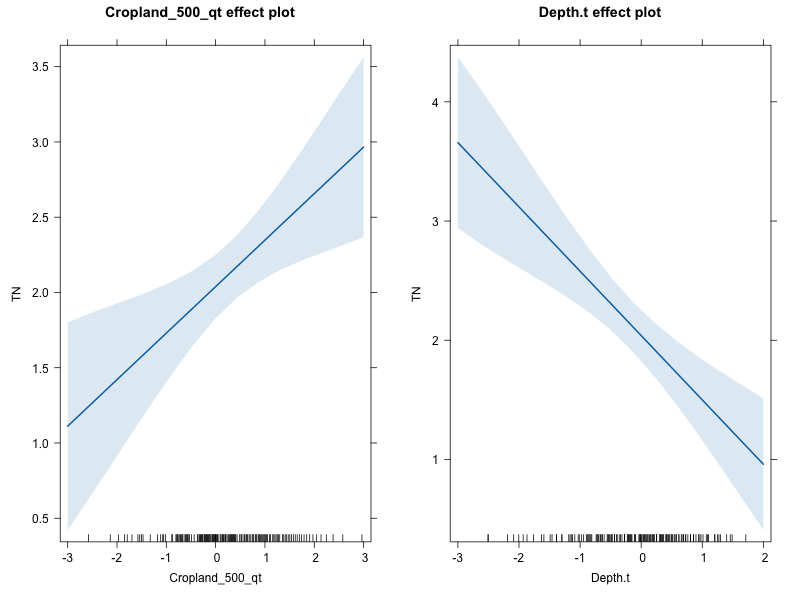
\includegraphics[width=1\linewidth]{tn_temp_glm_predictors.png}
 \caption{Enter Caption}
 
\end{figure}
\begin{figure}
 \centering
 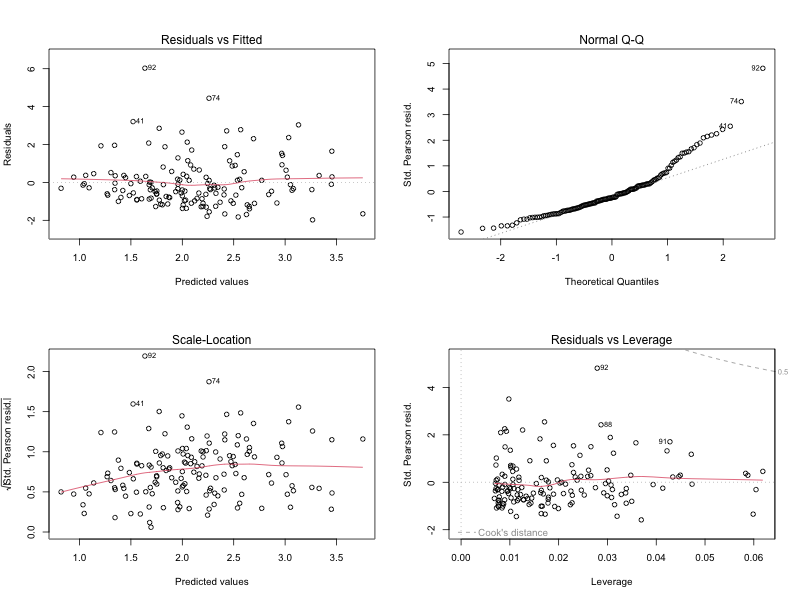
\includegraphics[width=1\linewidth]{tn_tempt_glm_diagnostics.png}
 \caption{Enter Caption}
 
\end{figure}

\subsubsection{3.2.2 Mediterranean regions}

GAM CHECK again
\begin{figure}
 \centering
 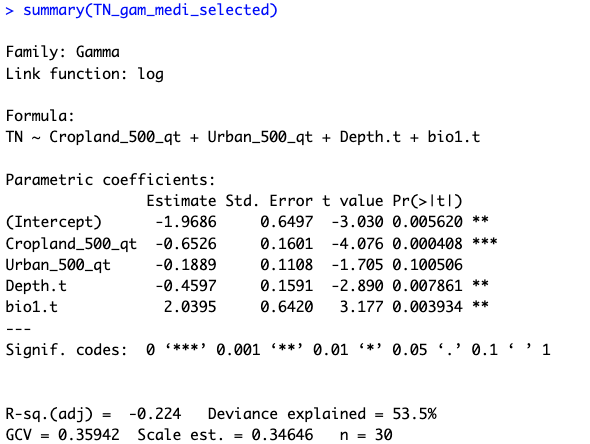
\includegraphics[width=0.75\linewidth]{tn_medi_gam_sum.png}
 \caption{Enter Caption}
 
\end{figure}
\begin{figure}
 \centering
 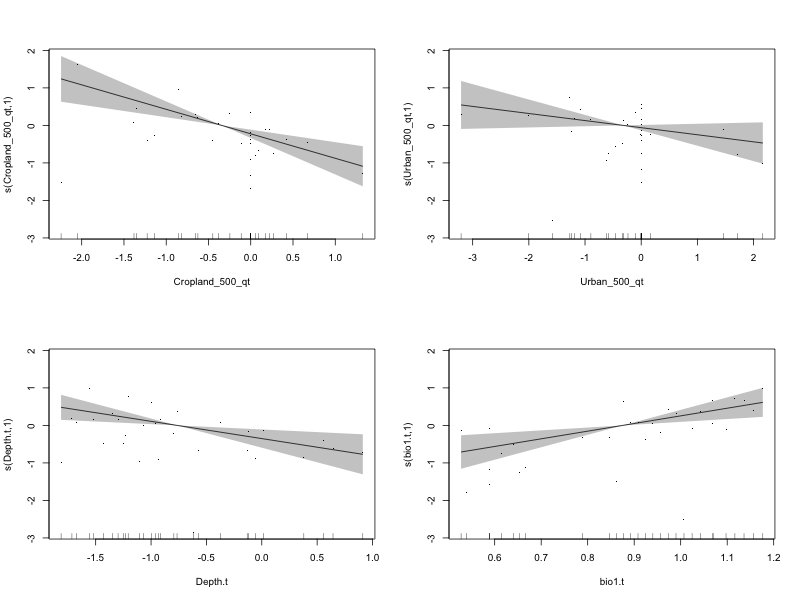
\includegraphics[width=1\linewidth]{tn_medi_gam_predictors.png}
 \caption{Enter Caption}
 
\end{figure}
\begin{figure}
 \centering
 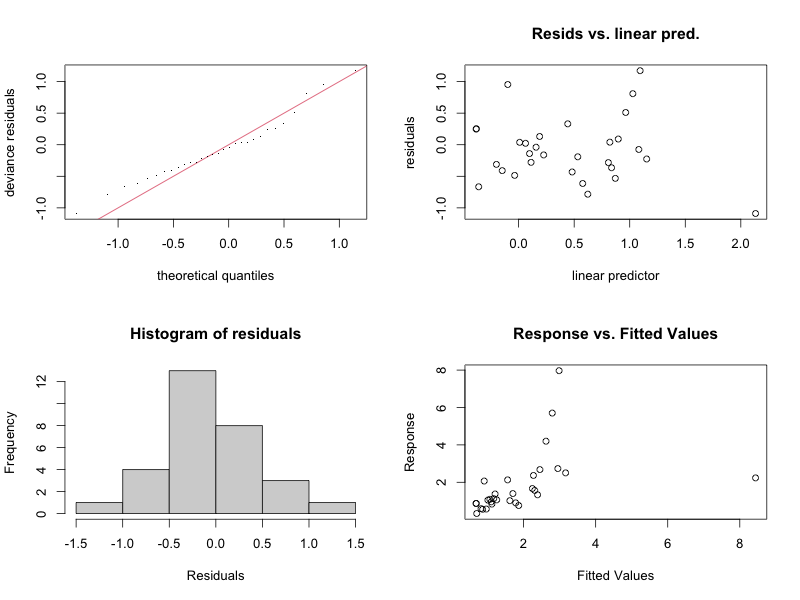
\includegraphics[width=1\linewidth]{tn_medi_gam_diagnostics.png}
 \caption{Enter Caption}
 
\end{figure}

GLM stepAIC chosen DEV 0.2283726 Adjusted R-squared: 0.1712

\begin{figure}
 \centering
 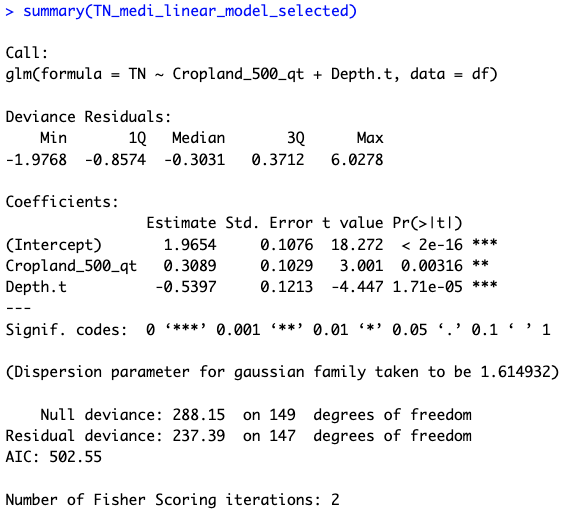
\includegraphics[width=0.75\linewidth]{tn_medi_glm_sum.png}

 
 \caption{Enter Caption}
 
\end{figure}
\begin{figure}
 \centering
 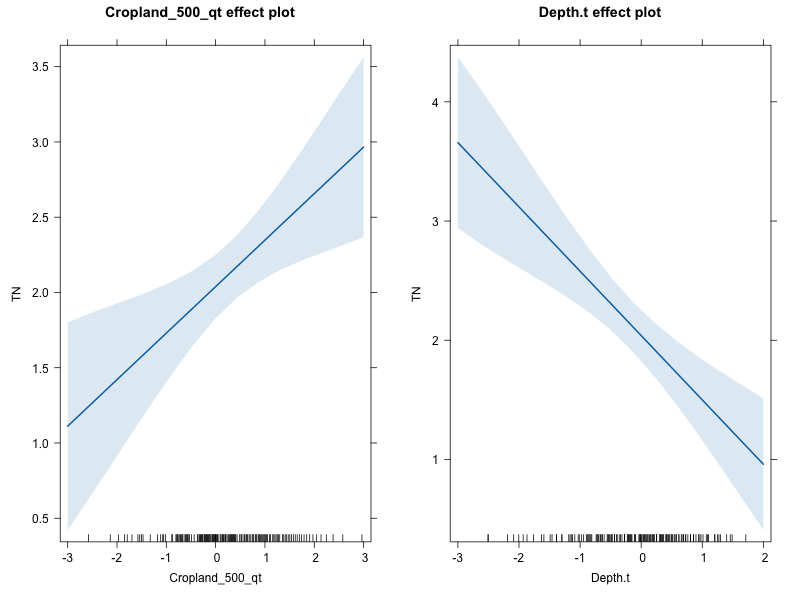
\includegraphics[width=1\linewidth]{tn_medi_glm_predictors.png}
\end{figure}
\begin{figure}
 \centering
 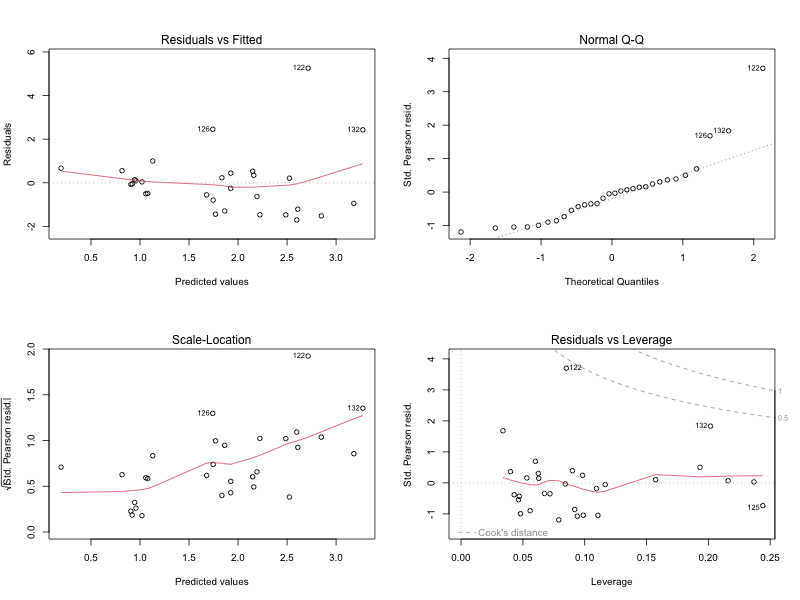
\includegraphics[width=1\linewidth]{tn_medi_glm_diagnostics.png}
 \caption{Enter Caption}
 
\end{figure}

\subsubsection{3.2.3 Continental regions}
\begin{figure}
 \centering
 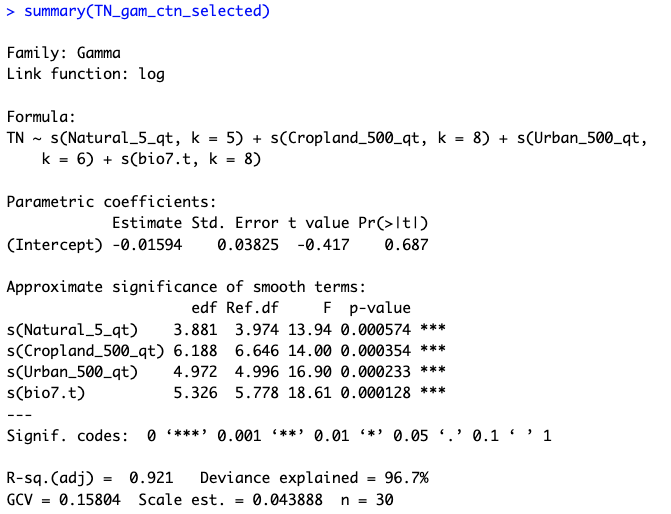
\includegraphics[width=0.75\linewidth]{tn_ctn_gam_sum.png}
 \caption{Enter Caption}
 
\end{figure}
\begin{figure}
 \centering
 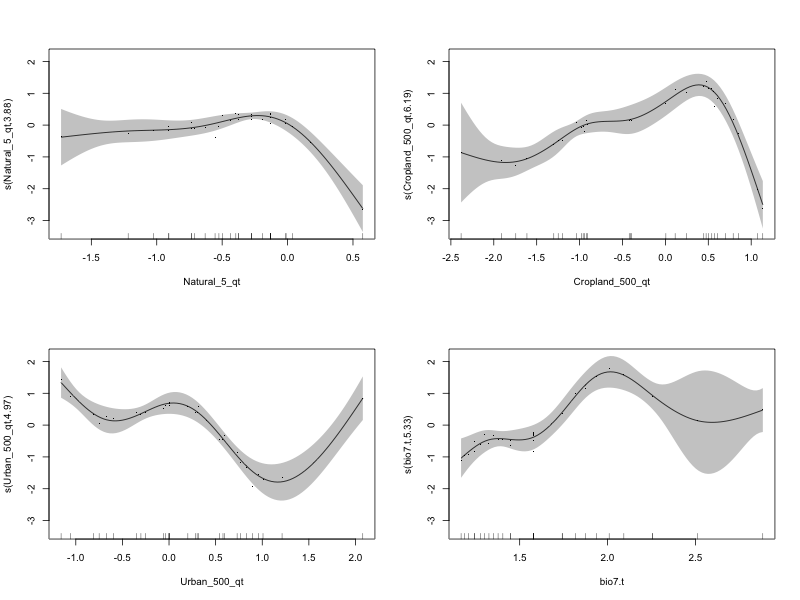
\includegraphics[width=1\linewidth]{tn_ctn_gam_predictors.png}
 \caption{Enter Caption}
 
\end{figure}
\begin{figure}
 \centering
 \includegraphics[width=1\linewidth]{tn_gam_diagnostics.png}
 \caption{Enter Caption}
 
\end{figure}
GLM\\ R2 0.05546 DEV 0.08802378
\begin{figure}
 \centering
 \includegraphics[width=0.75\linewidth]{tn_ctn_glm_sum.png}
 \caption{Enter Caption}
 
\end{figure}
\begin{figure}
 \centering
 \includegraphics[width=1\linewidth]{tn_ctn_glm_predictors.png}
 \caption{Enter Caption}
 
\end{figure}


\begin{figure}
 \centering
 \includegraphics[width=1\linewidth]{tn_ctn_glm_diagnostics.png}
 \caption{Enter Caption}
 
\end{figure}
\subsubsection{3.2.4 Subtropical regions}
GAM
\begin{figure}
 \centering
 \includegraphics[width=1\linewidth]{tn_subt_gam_sum_noselected.png}
 \caption{Enter Caption}
 
\end{figure}
\begin{figure}
 \centering
 \includegraphics[width=1\linewidth]{TN_subt_predictors.png}
 \caption{Enter Caption}
 
\end{figure}
\begin{figure}
 \centering
 \includegraphics[width=1\linewidth]{TN_subt_diagnostics.png}
 \caption{Enter Caption}
 
\end{figure}
GLM R2 0.1762 DEV0.2677453
\begin{figure}
 \centering
 \includegraphics[width=0.75\linewidth]{tn_subt_glm_sum.png}
 \caption{Enter Caption}
 
\end{figure}
\begin{figure}
 \centering
 \includegraphics[width=1\linewidth]{tn_subt_glm_diagnostics.png}
 \caption{Enter Caption}
 
\end{figure}

\begin{figure}
 \centering
 \includegraphics[width=1\linewidth]{tn_subt_glm_predictors.png}
 \caption{Enter Caption}
 
\end{figure}
\subsection{3.3 Log transformed response variables (log 10 found to be the best parameter)}

Bestnormalize package used for retrieving best parameter for log transformation
\subsubsection{TP}
TP general DEV 0.3599639 Adjusted R-squared:  0.3405  
Shapiro-Wilk normality test

data:  dev\_resid
W = 0.99036, p-value = 0.1156

\begin{figure}
    \centering
    \includegraphics[width=0.75\linewidth]{response_var_log_images/tp_log_glm_sum.png}
    \caption{Enter Caption}
    \label{fig:enter-label}
\end{figure}
\begin{figure}
    \centering
    \includegraphics[width=1\linewidth]{response_var_log_images/tp_log_glm_diagnostics.png}
    \caption{Enter Caption}
    \label{fig:enter-label}
\end{figure}
\begin{figure}
    \centering
    \includegraphics[width=1\linewidth]{response_var_log_images/tp_log_glm_predictors.png}
    \caption{Enter Caption}
    \label{fig:enter-label}
\end{figure}
mixed model  found by step 


R2m     R2c
0.1482045 0.37739
\(
log_TP ~ Aquatic_500_qt + Forest_500_qt + Depth.t + (1 | Country)
\)

We fitted a linear mixed model (estimated using REML and nloptwrap optimizer) to predict log_TP with Aquatic_500_qt, Forest_500_qt and
Depth.t (formula: log_TP ~ Aquatic_500_qt + Forest_500_qt + Depth.t). The model included Country as random effect (formula: ~1 |
Country). The model's total explanatory power is substantial (conditional R2 = 0.38) and the part related to the fixed effects alone
(marginal R2) is of 0.15. The model's intercept, corresponding to Aquatic_500_qt = 0, Forest_500_qt = 0 and Depth.t = 0, is at -0.81 (95\%
CI [-0.98, -0.63], t(232) = -9.10, p < .001). Within this model:

  - The effect of Aquatic 500 qt is statistically significant and negative (beta = -0.06, 95\% CI [-0.11, -6.34e-03], t(232) = -2.21, p =
0.028; Std. beta = -0.12, 95\% CI [-0.22, -0.01])
  - The effect of Forest 500 qt is statistically significant and negative (beta = -0.08, 95\% CI [-0.15, -0.02], t(232) = -2.42, p = 0.016;
Std. beta = -0.16, 95\% CI [-0.30, -0.03])
  - The effect of Depth t is statistically significant and negative (beta = -0.18, 95\% CI [-0.24, -0.12], t(232) = -5.82, p < .001; Std.
beta = -0.35, 95\% CI [-0.47, -0.23])

Standardized parameters were obtained by fitting the model on a standardized version of the dataset. 95\% Confidence Intervals (CIs) and
p-values were computed using a Wald t-distribution approximation.
\begin{figure}
    \centering
    \includegraphics[width=0.75\linewidth]{response_var_log_images/tp_log_mixed_sum.png}
    \caption{Enter Caption}
    \label{fig:enter-label}
\end{figure}
\begin{figure}
    \centering
    \includegraphics[width=1\linewidth]{response_var_log_images/tp_log_mixed_predictors.png}
    \caption{Enter Caption}
    \label{fig:enter-label}
\end{figure}

\begin{figure}
    \centering
    \includegraphics[width=1\linewidth]{response_var_log_images/tp_log_mixed_diagnostics.png}
    \caption{Enter Caption}
    \label{fig:enter-label}
\end{figure}



TP temp (0.4730498 DEV)  Adjusted R-squared:  0.4451 
\begin{figure}
    \centering
    \includegraphics[width=0.75\linewidth]{response_var_log_images/tp_log_temp_glm_sum.png}
    \caption{Enter Caption}
    \label{fig:enter-label}
\end{figure}
\begin{figure}
    \centering
    \includegraphics[width=1\linewidth]{response_var_log_images/tp_log_temp_glm_diagnostics.png}
    \caption{Enter Caption}
    \label{fig:enter-label}
\end{figure}
\begin{figure}
    \centering
    \includegraphics[width=1\linewidth]{response_var_log_images/tp_log_temp_glm_predictos.png}
    \caption{Enter Caption}
    \label{fig:enter-label}
\end{figure}
TP temperate mixed model  RANDOM effect not selected

\begin{figure}
    \centering
    \includegraphics[width=1\linewidth]{response_var_log_images/tp_log_temp_mixed_sum.png}
    \caption{Enter Caption}
    \label{fig:enter-label}
\end{figure}

TP medi (0.4633114 DEV)  Adjusted R-squared:  0.4451 
\begin{figure}
    \centering
    \includegraphics[width=0.75\linewidth]{response_var_log_images/tp_log_medi_sum.png}
    \caption{Enter Caption}
    \label{fig:enter-label}
\end{figure}
\begin{figure}
    \centering
    \includegraphics[width=1\linewidth]{response_var_log_images/tp_log_medi_glm_diagnostics.png}
    \caption{Enter Caption}
    \label{fig:enter-label}
\end{figure}
\begin{figure}
    \centering
    \includegraphics[width=1\linewidth]{response_var_log_images/tp_log_medi_glm_predictos.png}
    \caption{Enter Caption}
    \label{fig:enter-label}
\end{figure}
TP ctn (0.3250906 DEV) Adjusted R-squared:  0.2751 
\begin{figure}
    \centering
    \includegraphics[width=0.75\linewidth]{response_var_log_images/tp_log_ctn_glm_sum.png}
    \caption{Enter Caption}
    \label{fig:enter-label}
\end{figure}
\begin{figure}
    \centering
    \includegraphics[width=1\linewidth]{response_var_log_images/tp_log_ctn_glm_diagnostics.png}
    \caption{Enter Caption}
    \label{fig:enter-label}
\end{figure}
\begin{figure}
    \centering
    \includegraphics[width=1\linewidth]{response_var_log_images/tp_log_ctn_glm_predictos.png}
    \caption{Enter Caption}
    \label{fig:enter-label}
\end{figure}
TP subp (0.4306284 DEV) Adjusted R-squared:  0.3595 

\begin{figure}
    \centering
    \includegraphics[width=0.75\linewidth]{response_var_log_images/tp_log_subp_glm_sum.png}
    \caption{Enter Caption}
    \label{fig:enter-label}
\end{figure}
\begin{figure}
    \centering
    \includegraphics[width=1\linewidth]{response_var_log_images/tp_log_subp_glm_diagnostics.png}
    \caption{Enter Caption}
    \label{fig:enter-label}
\end{figure}
\begin{figure}
    \centering
    \includegraphics[width=1\linewidth]{response_var_log_images/tp_log_subp_glm_predictos.png}
    \caption{Enter Caption}
    \label{fig:enter-label}
\end{figure}
\subsubsection{TN}
TN general 0.2867796 DEV Adjusted R-squared:  0.2589 
\begin{figure}
    \centering
    \includegraphics[width=0.75\linewidth]{response_var_log_images/TN_log_glm_sum.png}
    \caption{Enter Caption}
    \label{fig:enter-label}
\end{figure}
\begin{figure}
    \centering
    \includegraphics[width=1\linewidth]{response_var_log_images/TN_log_glm_diagnostics.png}
    \caption{Enter Caption}
    \label{fig:enter-label}
\end{figure}
\begin{figure}
    \centering
    \includegraphics[width=1\linewidth]{response_var_log_images/TN_log_glm_predictors.png}
    \caption{Enter Caption}
    \label{fig:enter-label}
\end{figure}
TN mixed effect general

We fitted a linear mixed model (estimated using REML and nloptwrap optimizer) to predict log_TN with Forest_500_qt, Area.t and Depth.t
(formula: log_TN ~ Forest_500_qt + Area.t + Depth.t). The model included Country as random effect (formula: ~1 | Country). The model's
total explanatory power is substantial (conditional R2 = 0.37) and the part related to the fixed effects alone (marginal R2) is of 0.10.
The model's intercept, corresponding to Forest_500_qt = 0, Area.t = 0 and Depth.t = 0, is at 0.15 (95\% CI [0.04, 0.27], t(232) = 2.70, p
= 0.007). Within this model:

  - The effect of Forest 500 qt is statistically significant and negative (beta = -0.06, 95\% CI [-0.10, -0.02], t(232) = -2.80, p = 0.006;
Std. beta = -0.19, 95\% CI [-0.33, -0.06])
  - The effect of Area t is statistically significant and positive (beta = 0.06, 95\% CI [0.02, 0.09], t(232) = 3.40, p < .001; Std. beta =
0.19, 95\% CI [0.08, 0.30])
  - The effect of Depth t is statistically significant and negative (beta = -0.08, 95\% CI [-0.12, -0.04], t(232) = -4.16, p < .001; Std.
beta = -0.26, 95\% CI [-0.39, -0.14])

Standardized parameters were obtained by fitting the model on a standardized version of the dataset. 95\% Confidence Intervals (CIs) and
p-values were computed using a Wald t-distribution approximation.

\begin{figure}
    \centering
    \includegraphics[width=0.75\linewidth]{response_var_log_images/TN_log_mixed_sum.png}
    \caption{Enter Caption}
    \label{fig:enter-label}
\end{figure}

\begin{figure}
    \centering
    \includegraphics[width=1\linewidth]{response_var_log_images/TN_log_mixed_diagnostics.png}
    \caption{Enter Caption}
    \label{fig:enter-label}
\end{figure}
\begin{figure}
    \centering
    \includegraphics[width=1\linewidth]{response_var_log_images/TN_log_mixed_predictors.png}
    \caption{Enter Caption}
    \label{fig:enter-label}
\end{figure}

TN medi  0.5140397 DEV Adjusted R-squared:  0.4363 
\begin{figure}
    \centering
    \includegraphics[width=0.75\linewidth]{response_var_log_images/TN_log_medi_glm_sum.png}
    \caption{Enter Caption}
    \label{fig:enter-label}
\end{figure}
\begin{figure}
    \centering
    \includegraphics[width=1\linewidth]{response_var_log_images/TN_log_medi_glm_diagnostics.png}
    \caption{Enter Caption}
    \label{fig:enter-label}
\end{figure}
\begin{figure}
    \centering
    \includegraphics[width=1\linewidth]{response_var_log_images/TN_log_medi_glm_predictors.png}
    \caption{Enter Caption}
    \label{fig:enter-label}
\end{figure}
TN temp 0.3087187 Adjusted R-squared: DEV 0.2797 
\begin{figure}
    \centering
    \includegraphics[width=0.75\linewidth]{response_var_log_images/TN_log_temp_sum.png}
    \caption{Enter Caption}
    \label{fig:enter-label}
\end{figure}
\begin{figure}
    \centering
    \includegraphics[width=1\linewidth]{response_var_log_images/TN_log_temp_glm_diagnostics.png}
    \caption{Enter Caption}
    \label{fig:enter-label}
\end{figure}
\begin{figure}
    \centering
    \includegraphics[width=1\linewidth]{response_var_log_images/TN_log_temp_glm_predictors.png}
    \caption{Enter Caption}
    \label{fig:enter-label}
\end{figure}
TN temp mixed
 R2m       R2c
[1,] 0.06058967 0.2931516

\begin{figure}
    \centering
    \includegraphics[width=0.75\linewidth]{response_var_log_images/TN_log_temp_mixed_sum.png}
    \caption{Enter Caption}
    \label{fig:enter-label}
\end{figure}

\begin{figure}
    \centering
    \includegraphics[width=1\linewidth]{response_var_log_images/TN_log_temp_mixed_diagnostics.png}
    \caption{Enter Caption}
    \label{fig:enter-label}
\end{figure}
\begin{figure}
    \centering
    \includegraphics[width=1\linewidth]{response_var_log_images/TN_log_temp_mixed_predictors.png}
    \caption{+}
    \label{fig:enter-label}
\end{figure}
TN ctn DEV 0.1990106 Adjusted R-squared:  0.1066 
\begin{figure}
    \centering
    \includegraphics[width=0.75\linewidth]{response_var_log_images/TN_log_ctn_glm_sum.png}
    \caption{Enter Caption}
    \label{fig:enter-label}
\end{figure}
\begin{figure}
    \centering
    \includegraphics[width=1\linewidth]{response_var_log_images/TN_log_ctn_glm_diagnostics.png}
    \caption{Enter Caption}
    \label{fig:enter-label}
\end{figure}
\begin{figure}
    \centering
    \includegraphics[width=1\linewidth]{response_var_log_images/TN_log_ctn_glm_predictors.png}
    \caption{Enter Caption}
    \label{fig:enter-label}
\end{figure}
TN subtropical DEV 0.21614  Adjusted R-squared:  0.1534 
\begin{figure}
    \centering
    \includegraphics[width=0.75\linewidth]{response_var_log_images/TN_log_subp_glm_sum.png}
    \caption{Enter Caption}
    \label{fig:enter-label}
\end{figure}
\begin{figure}
    \centering
    \includegraphics[width=1\linewidth]{response_var_log_images/TN_log_subp_glm_diagnostics.png}
    \caption{Enter Caption}
    \label{fig:enter-label}
\end{figure}
\begin{figure}
    \centering
    \includegraphics[width=1\linewidth]{response_var_log_images/TN_log_subp_glm_predictors.png}
    \caption{Enter Caption}
    \label{fig:enter-label}
\end{figure}
\section{References}
\bibliographystyle{plain}
\bibliography{bibliography}



\end{document}

